

\subsection{Versuchsbedingungen}

Um im Rahmen der Versuchsauswertung im \Abschnitt\ref{cha:4_Auswertung} eine Validierung des Teststandes vornehmen zu können, wurden vor allem Messungen mit Leiterplatten durchgeführt, die mit frequenzselektiven Oberflächen gefertigt wurden. Für diese Proben existieren Vergleichsmessungen hoher Qualität vom Institut für Nachrichtentechnik der TUD~\cite{FSS_Toedter_Diplomarbeit}. Da die Änderung der elektrischen Leitfähigkeit der Leiterbahnen, welche für die Schirmdämpfung nicht magnetischer Materialien bei gegebener Frequenz vor allem ausschlaggebend ist (vgl. \Abschnitt\ref{cha:2_sub_Schirmung_ebener_Wellenfelder}), aufgrund von Schwankungen der Umgebungsbedingungen in den Laborräumen vernachlässigbar ist~\cite{Materialdaten_Kupfer}, ist vor allem die Sensitivität des VNA gegenüber wechselnden Betriebstemperaturen zu beachten.
\par
\vspace{\linespace}
Um vergleichbare Messungen über der gesamten Messdauer zu erhalten, wurden diese zur Verringerung von Temperaturdrifts erst nach einer ausreichenden Aufwärmzeit des VNA durchgeführt (vgl. \Abschnitt\ref{cha:4_Kalibration_Messtechnik}). Die Betriebsbedingungen in den Laborräumen entsprechend des Weiteren weitestgehend denen der Erstkalibration und Einrichtung des VNA beim Hersteller laut des entsprechenden Protokolls. Es kann somit davon ausgegangen werden, dass die Abweichungen zwischen einzelnen Messungen durch Temperaturschwankungen minimal sind. Für die verwendeten Pyramidenabsorber gilt außerdem die angegebene garantierte Reflektionsdämpfung in einem weiten Temperaturbereich, sodass auch hier keine großen Schwankungen zu erwarten sind~\cite{Eco_Messtechnik_Absorber}.
%Tempraturabhängigkeit Absorber

%Versuchsbedingungen --> siehe Prjektarbeit


\subsection{Versuchsvorbereitung}

Die abschließenden Vorbereitungen vor der Durchführung der Messungen beinhalteten neben dem Anschluss aller Signalkabel und des VNA auch das Aufstellen der Antennen und die Platzierung des Reflektors so, dass eine direkte Sichtverbindung beider Antennen nur durch die Probenöffnung möglich ist. Da es sich bei den Antennen um Richtantennen handelt, ist die Ausrichtung zueinander unter Beachtung der Polarisationsrichtung von besonderer Bedeutung. Dies wurde durch sorgfältige Vermessung sichergestellt, ebenso wie die vertikale Ausrichtung des Reflektors entsprechend der gestellten Anforderungen. Die aufgebaute Messstrecke ist in der \Abb\ref{fig:4_Messstrecke} zu sehen.
\par
\vspace{\linespace}

\begin{figure}[ht]
    \centering
    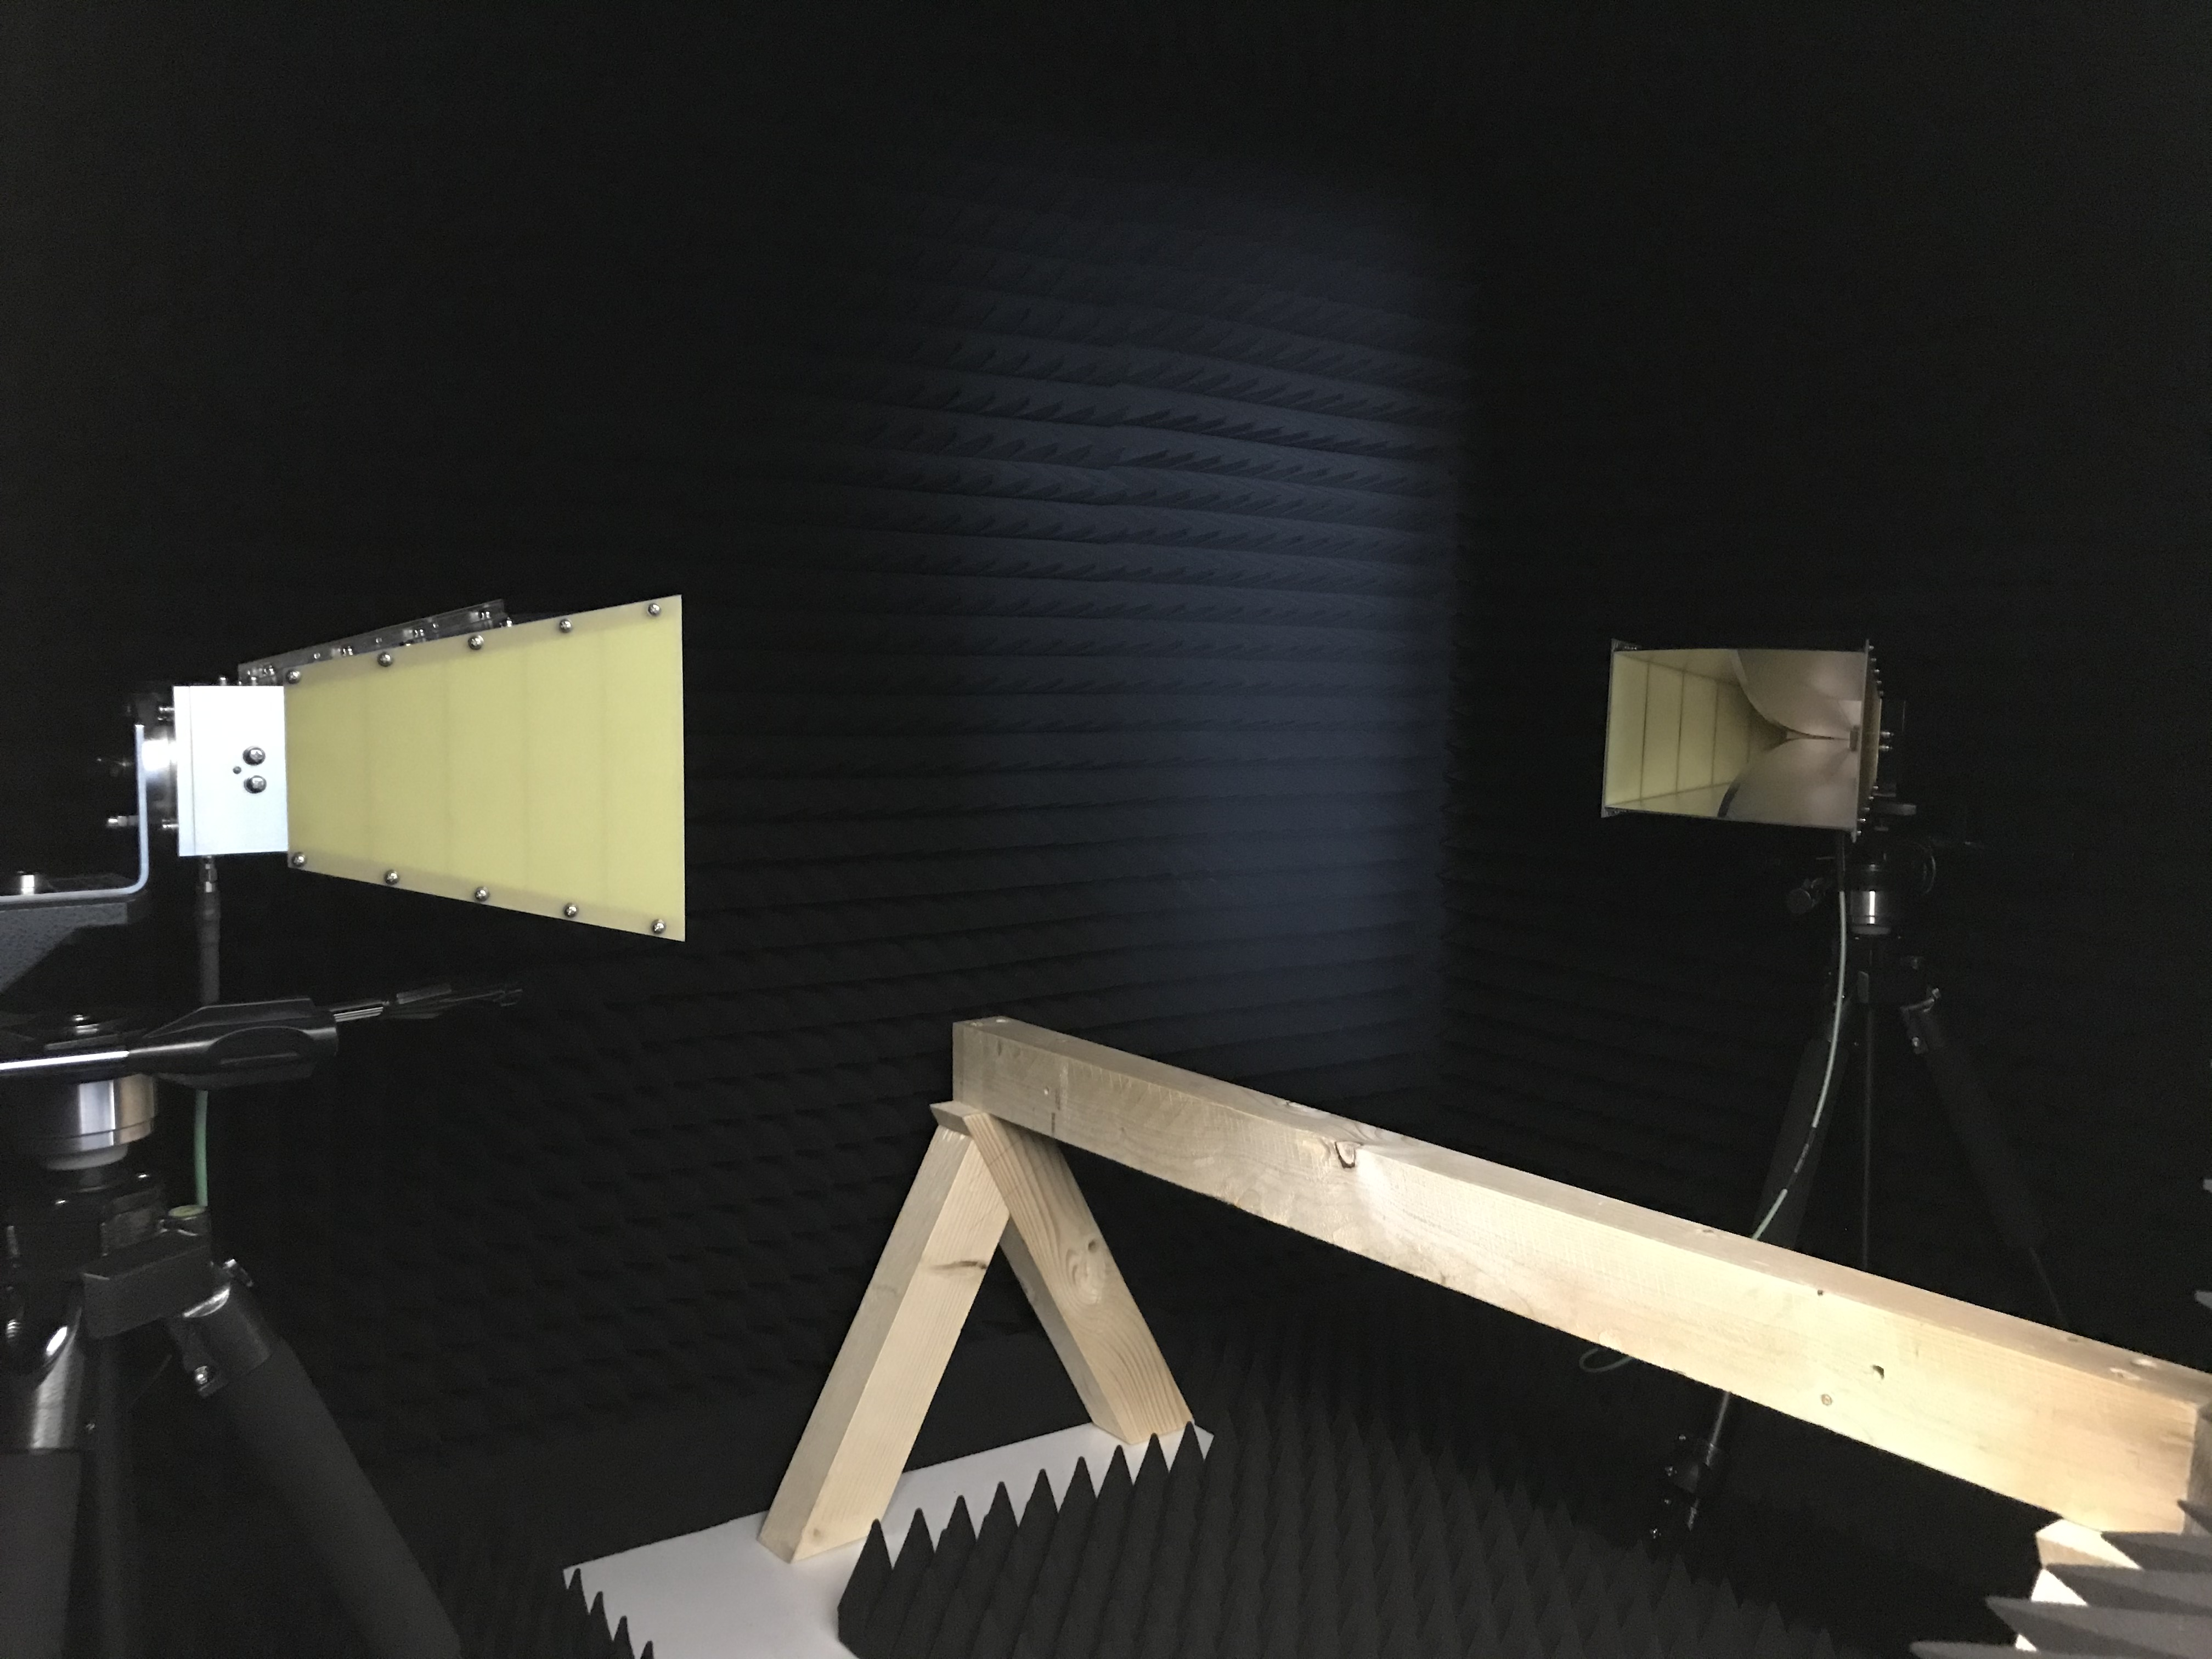
\includegraphics[height=.2\textheight, draft = false]{Abbildungen/Kapitel4/IMG_5660.jpg}
    \hspace{1cm}
    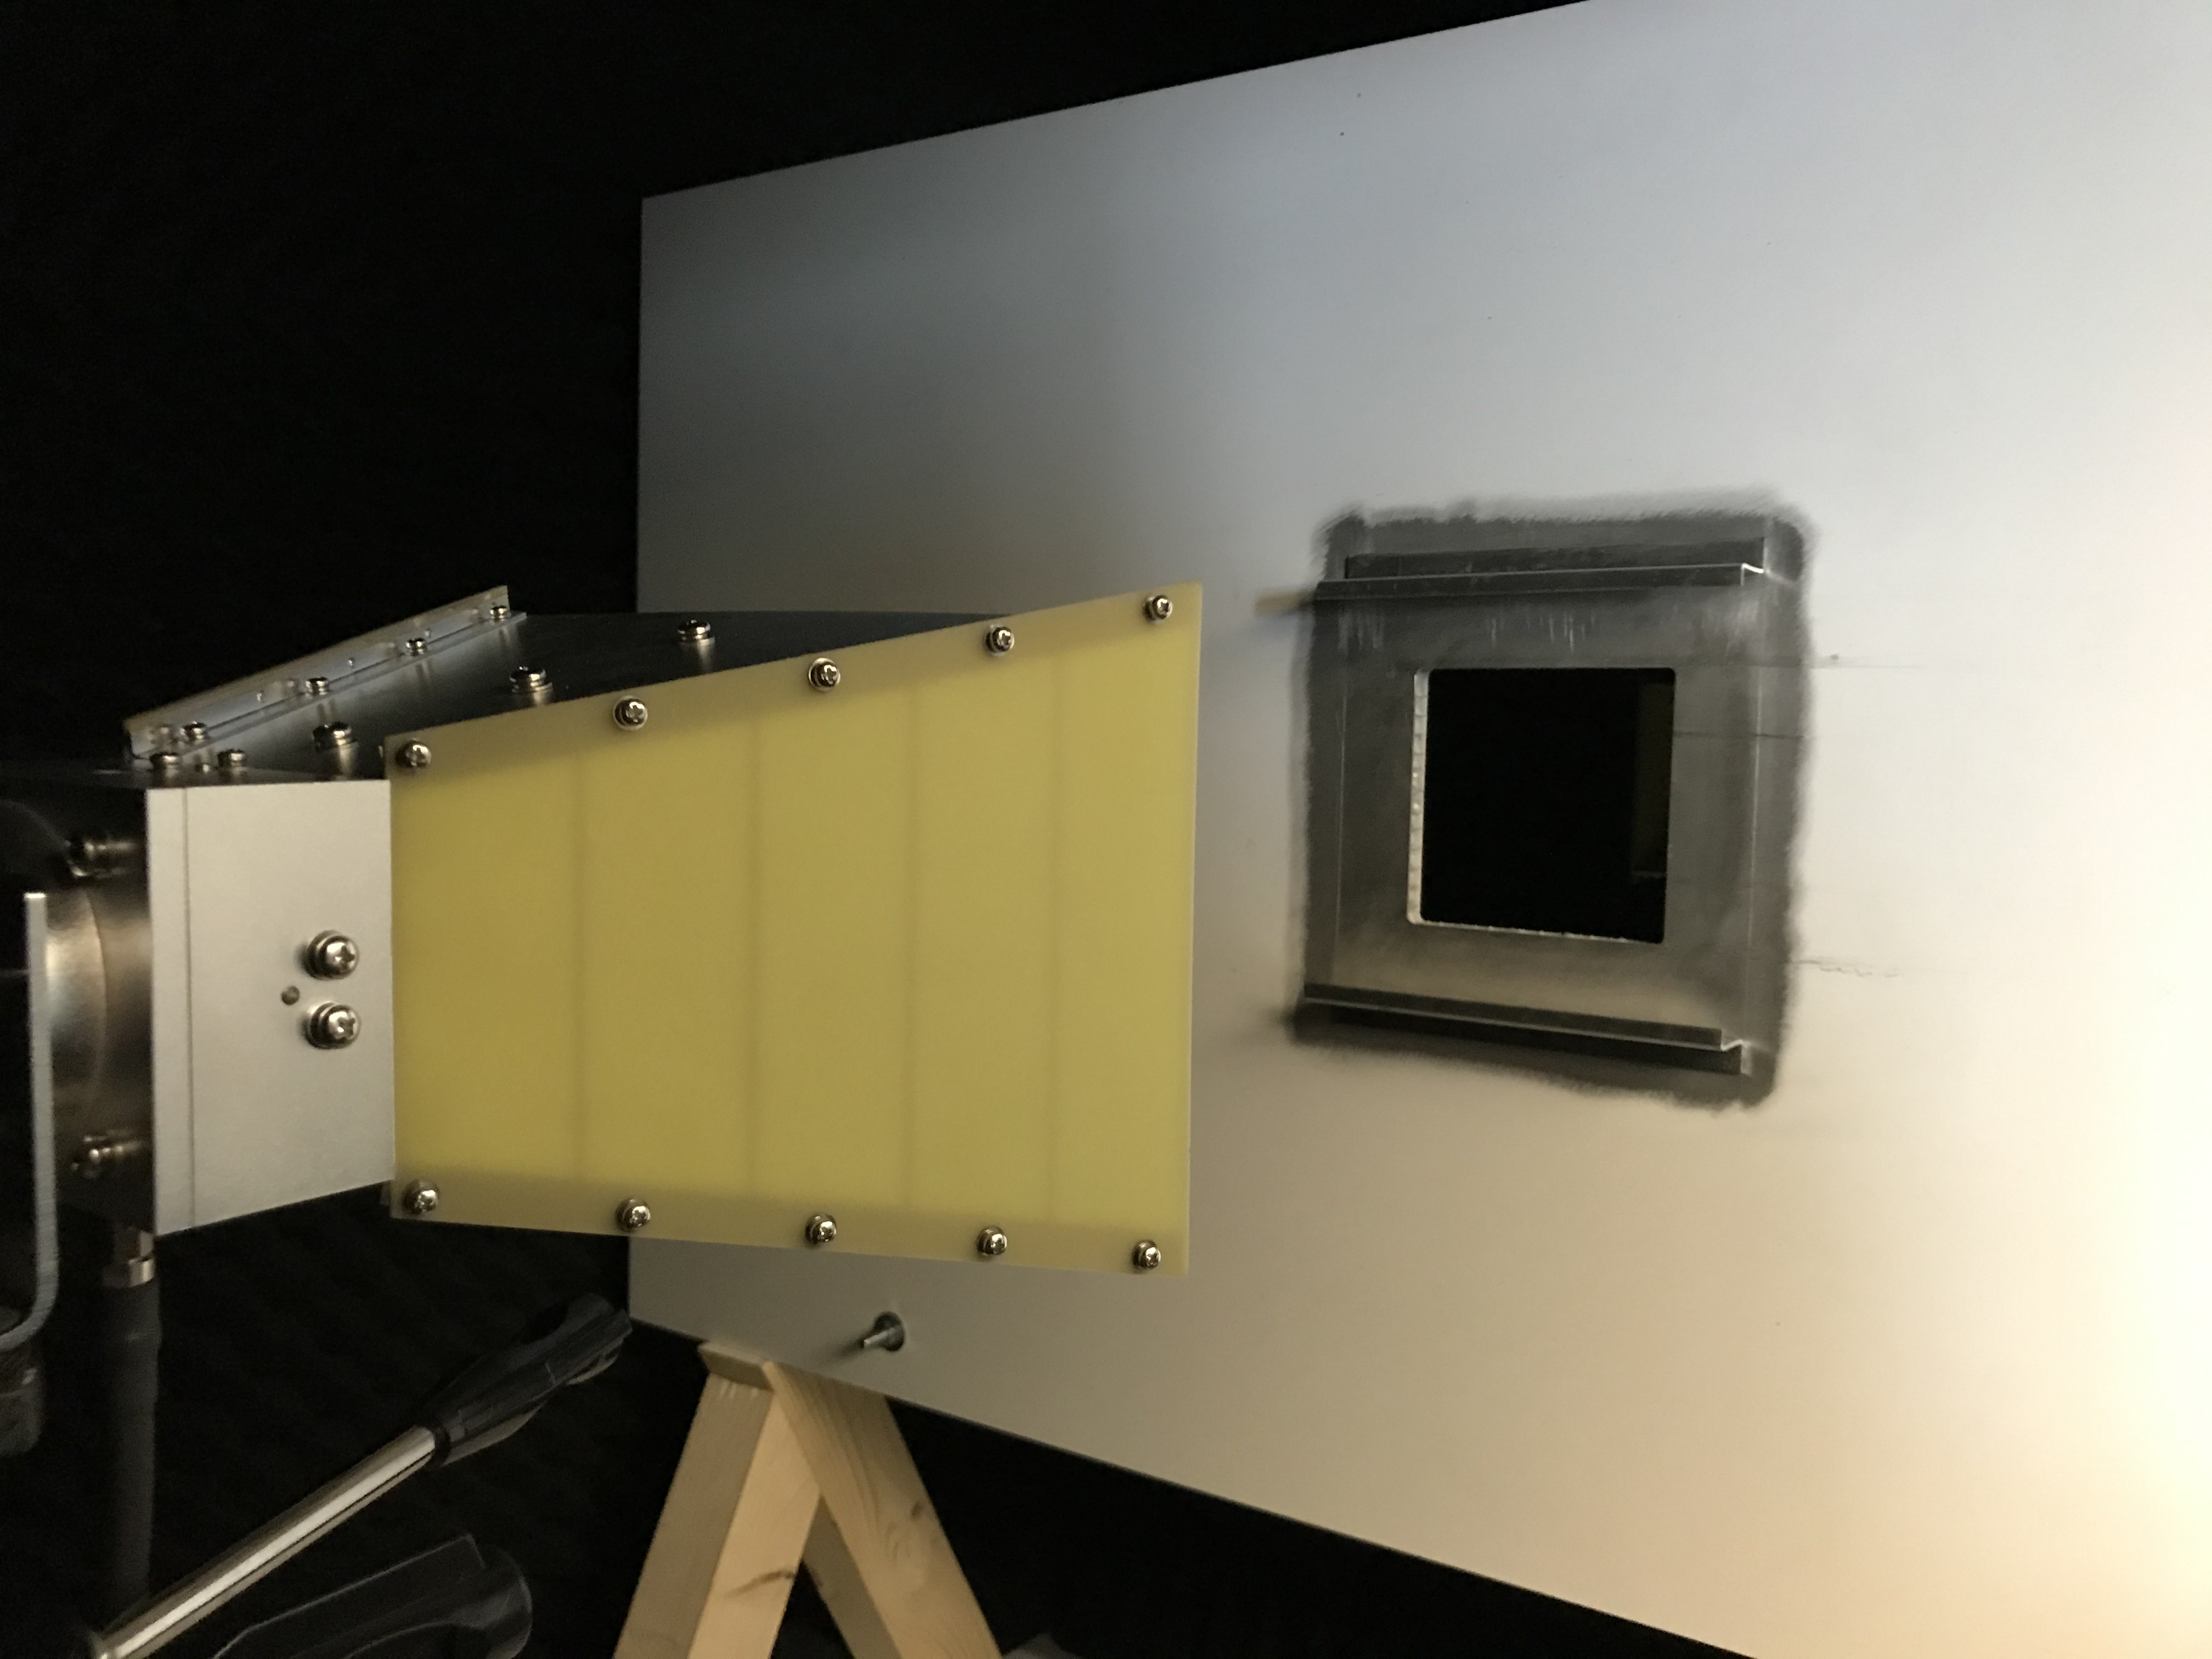
\includegraphics[height=.2\textheight, draft = false]{Abbildungen/Kapitel4/IMG_5665.jpg}
    \caption{Messstrecke ohne und mit Reflektor}
    \label{fig:4_Messstrecke}
\end{figure}


%Ausrichtung der Antennen genau
%Ebene der Probekörper genau


Ein weiterer wichtiger Schritt der Versuchsvorbereitung ist die korrekte Verbindung aller Signalkabel mit den entsprechenden Konnektoren, sowohl zur Kalibration als auch für die eigentlichen Messungen. Durch eine unsaubere Verschraubung an der Schnittstelle zweier Kabel steigt der Wellenwiderstand, sodass aufgrund des Impedanzsprungs eine Grenzfläche entsteht. Dies führt entsprechend den Betrachtungen in \Abschnitt\ref{cha:2_sub_Verhalten_an_Grenzflächen} zu ungewollten Reflektionen innerhalb der Signalleitung und kann das Messsignal störend beeinflussen. Häufig ist eine schlechte Verbindung auch an einem instabilen Signal zu erkennen. Bei der Verschraubung ist daher stets auf die korrekte Ausrichtung der Konnektoren zueinander zu achten und die Verbindung ist nach vorsichtigem Anziehen per Hand mittels eines Drehmomentenschlüssels unter Verwendung des korrekten Drehmoments zu sichern.
\par
\vspace{\linespace}
Abschließend wurde die gesamte Schirmhülle an der dafür vorgesehenen Adapterplatte, an der sich auch die Konnektoren der Signalkabel befinden, mit Erdpotenzial verbunden. Dadurch können entstehende Störströme abgeleitet werden, sodass die Schirmungseffektivität dadurch nicht beeinträchtigt wird. 
\par
\vspace{\linespace}
Im Folgenden soll der allgemeine Ablauf einer vollständigen Messung, der für alle untersuchten Probetypen gleich ist, anhand der durchzuführenden Schritte dargestellt werden. 


\subsection{Versuchsdurchführung}

Zu Beginn jeder Messreihe wird eine kurze Sichtinspektion der Testkammer durchgeführt, um fehlerhafte Messergebnisse aufgrund von Beschädigungen oder Defekten schon zu Beginn ausschließen zu können. Im Anschluss erfolgt die Vorbereitung der Messung in der Shockline Software des VNA. Dies schließt die Kalibration der Messtechnik entsprechend den Ausführungen in \Abschnitt\ref{cha:4_Kalibration_Messtechnik} ein.
\par
\vspace{\linespace}
Nach Abschluss der Vorbereitungen kann die Messung der sogenannten Freiraumdämpfung erfolgen. Das bedeutet, dass die Schirmdämpfung der Messstrecke einschließlich des Probenhalters jedoch ohne Probe ermittelt wird. Dabei ist sicherzustellen, dass die beiden Teile des Probenhalters trotzdem fest miteinander verschraubt sind. Ist dies erfolgt, kann die Probe eingebracht werden. Auch hier ist zur Herstellung eines leitfähigen Kontaktes am gesamten Rand des Probekörpers mit dem Probenhalter auf eine feste Verschraubung zu achten. Um dies zu gewährleisten, wurden die vermessenen Leiterplatten bspw. mit Aluminiumband umklebt. Die eingebaute Probe ist in \Abb\ref{fig:4_Probenhalter_mit_Probe} zu sehen. Dort ist ebenfalls die Struktur zu erkennen, welche für eine frequenzselektive Dämpfung der Transmission sorgt. Diese besteht bei den vorliegenden Probekörpern im Wesentlichen aus kreuzförmigen Mustern unterschiedlicher Balkenbreite und -länge, welche die leitfähige Schicht der Leiterplatten unterbrechen. Für eine detaillierte Betrachtung der Wirkungsweise solcher frequenzselektiven Oberflächen sei auf die Arbeit~\cite{FSS_Toedter_Diplomarbeit} verwiesen.
\par
\vspace{\linespace}


\begin{figure}[ht]
    \centering
    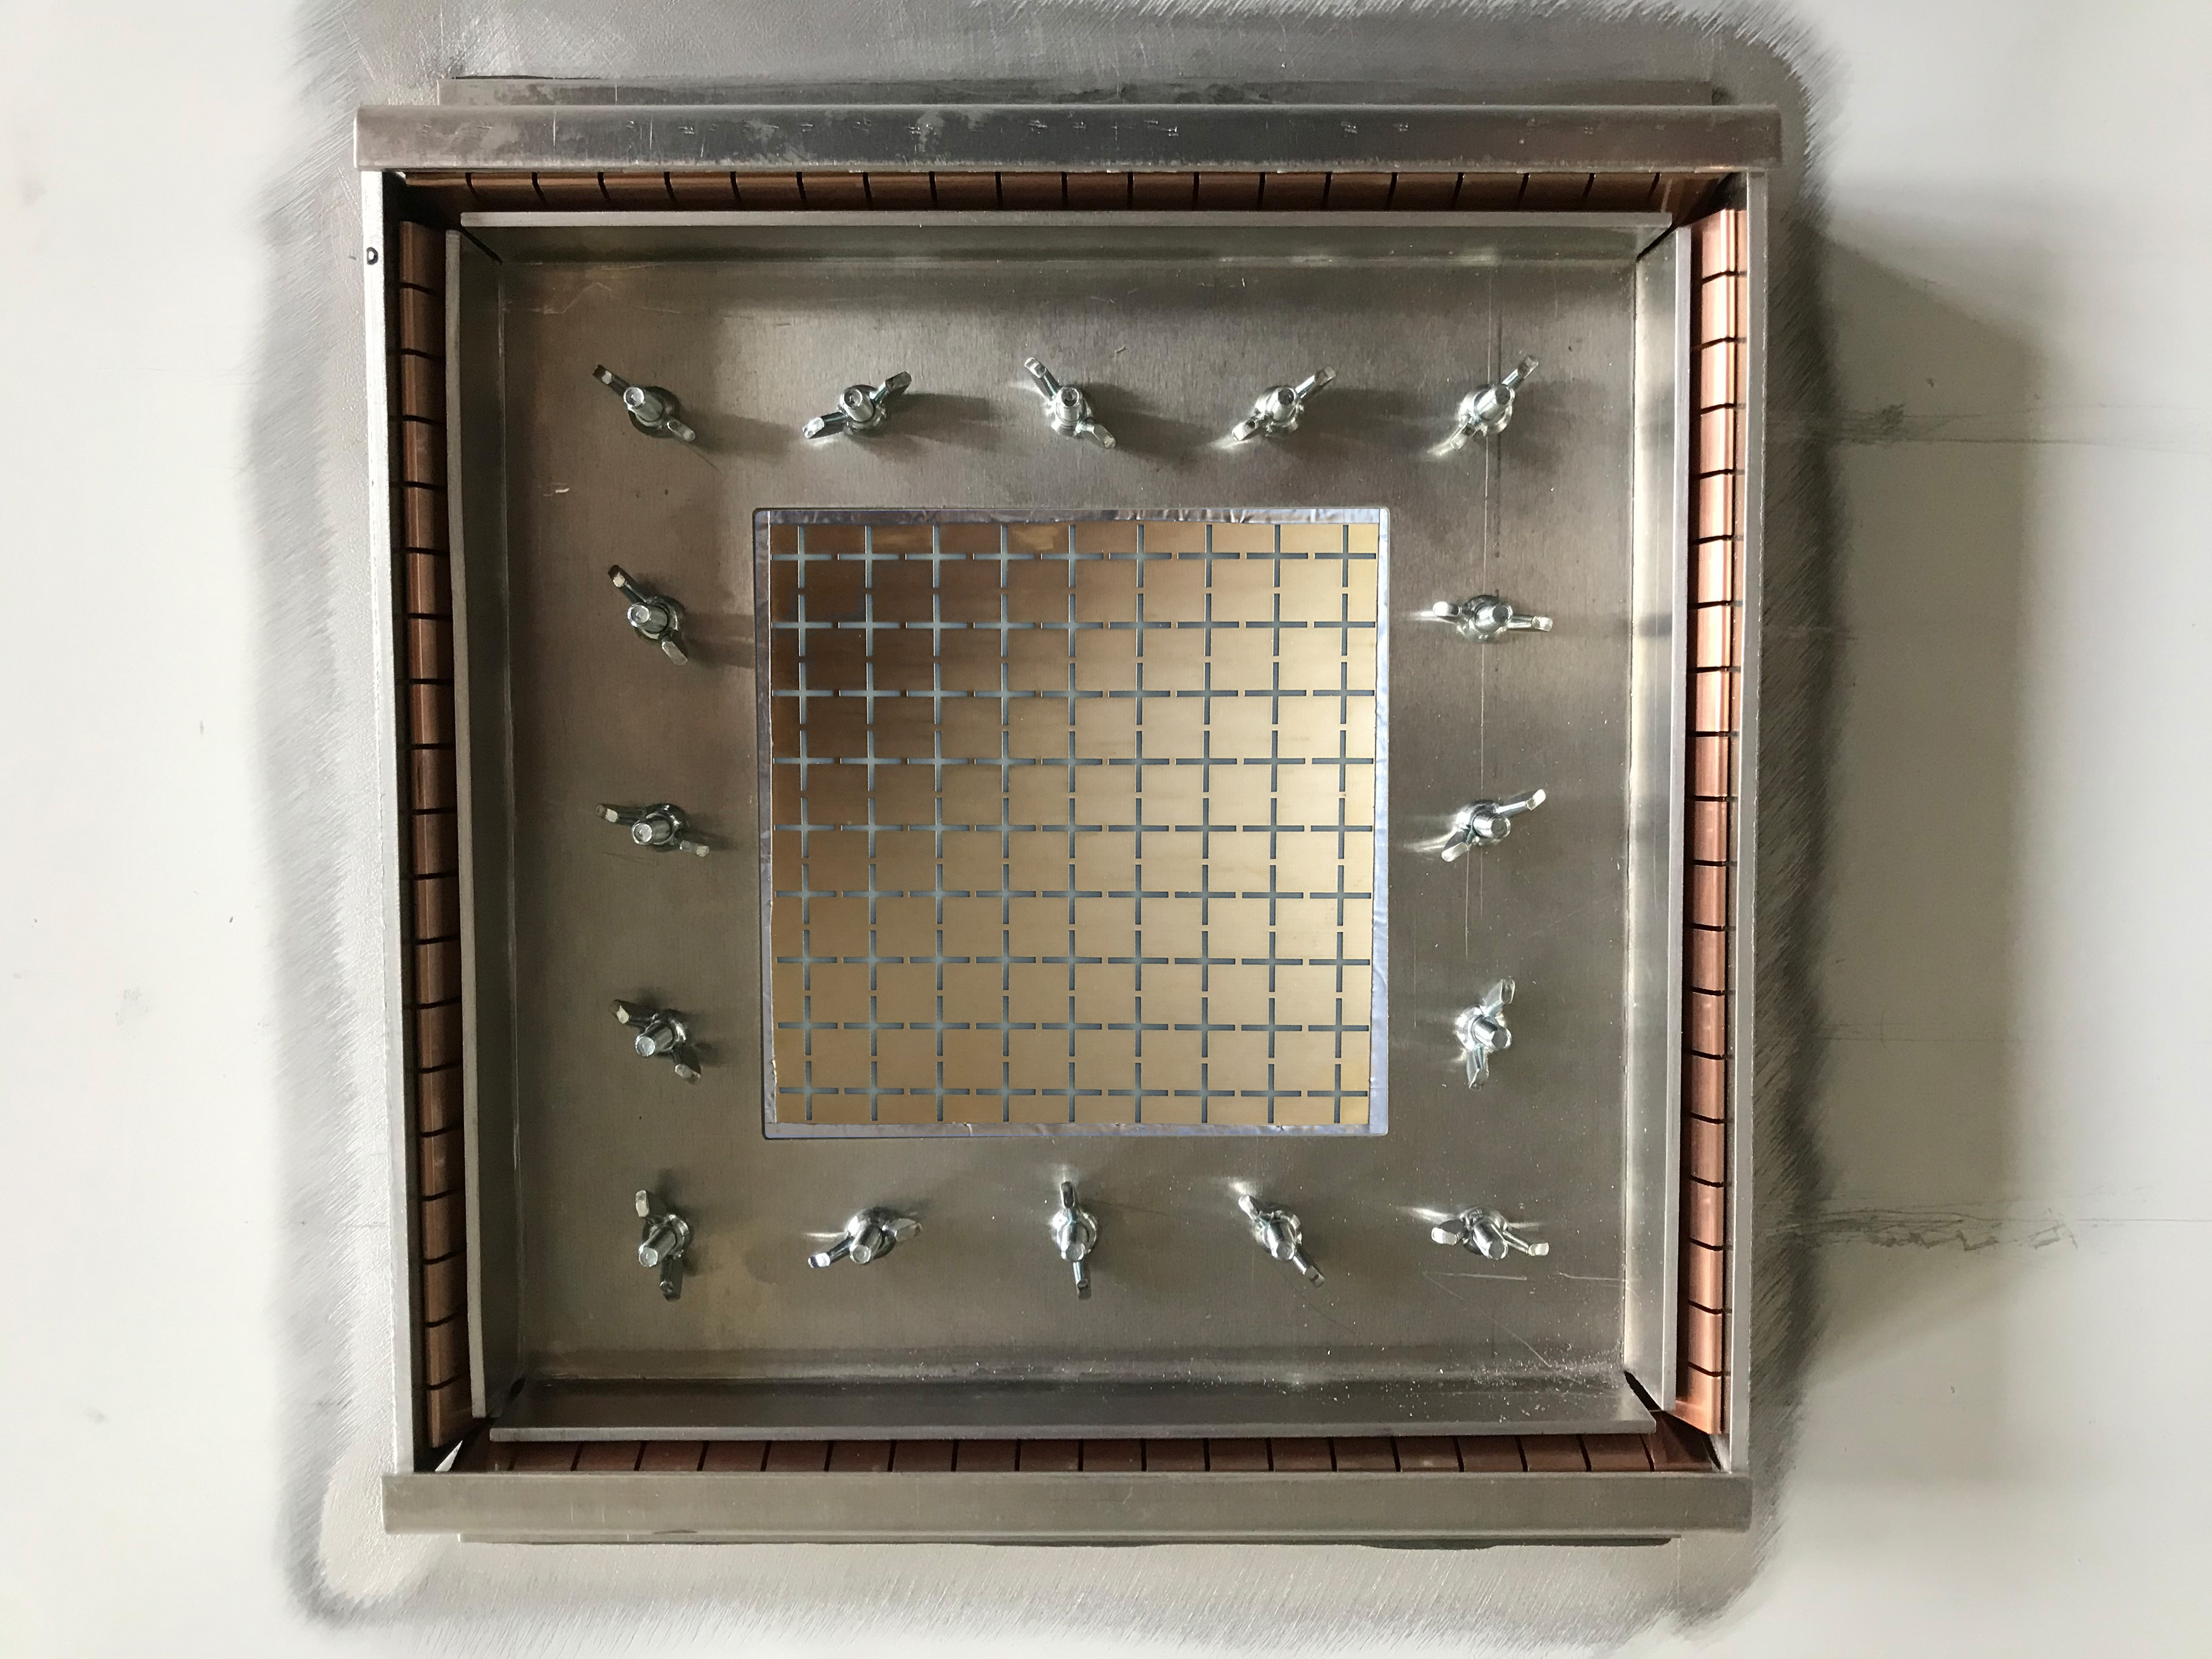
\includegraphics[height=.2\textheight, draft = false]{Abbildungen/Kapitel4/Probenhalter.jpg}
    \hspace{1cm}
    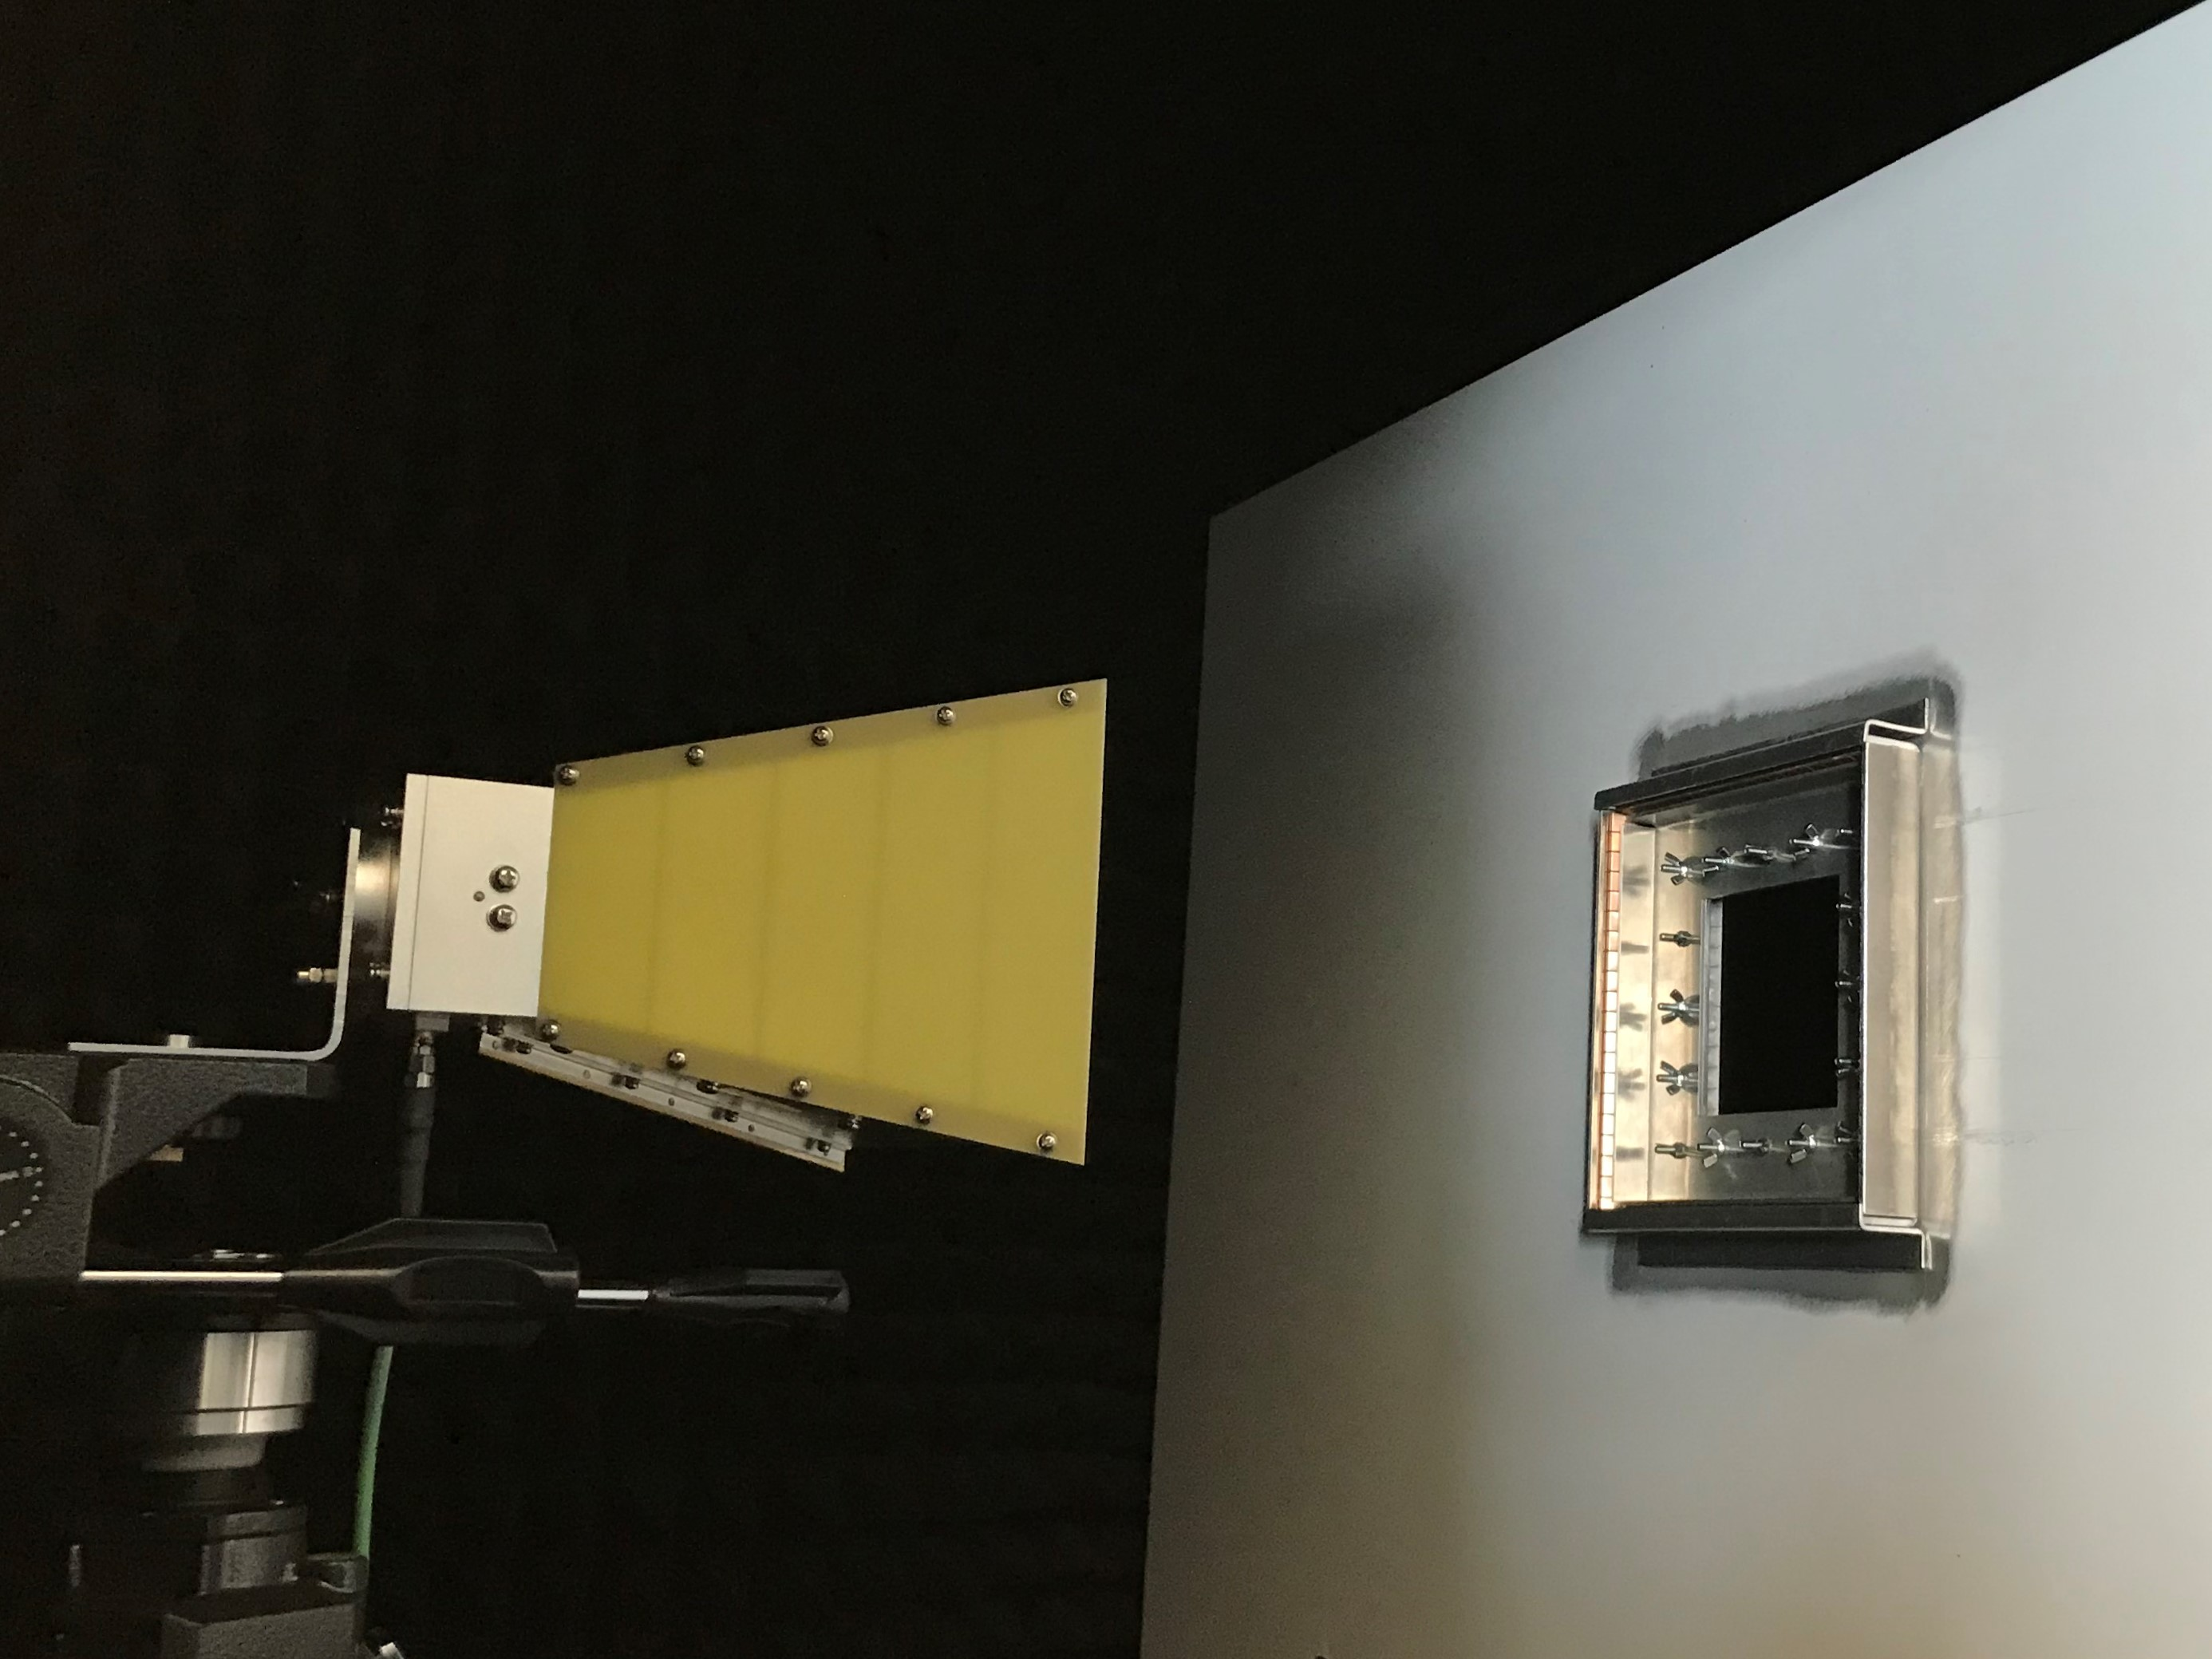
\includegraphics[height=.2\textheight, draft = false]{Abbildungen/Kapitel4/IMG_5675_trimmed.jpg}
    \caption{Probenhalter mit eingebauter Probe und Messstrecke mit Probenhalter}
    \label{fig:4_Probenhalter_mit_Probe}
\end{figure}


Die Ermittlung der S-Parameter mit Probe erfolgt analog zur Messung der Freiraumdämpfung. Die Einfüge- oder Schirmdämpfung kann dann durch Subtraktion der Dämpfung der Messstrecke von der ermittelten Gesamtdämpfung mit Probe berechnet werden (vgl. \Abschnitt\ref{cha:4_Allgemeines}). Zu beachten ist dabei, in welcher Reihenfolge die Ports des VNA an die Antennen angeschlossen wurden, sodass aus den gespeicherten Messwerten der korrekte Transmissionskoeffizient zur Berechnung der Schirmdämpfung genutzt wird.
\par
\vspace{\linespace}
Im folgenden \Abschnitt werden die Ergebnisse der durchgeführten Messungen ausgewertet.




%Verschraubung Probenhalter

%Messung ohne Probe

%Verschraubung Probe

%Messung mit Probe

%Differenz beider Messungen = S21






